\chapter{Related Work}

\section{Pose Estimation}
first: single images only, no video
\subsection{Pictoral Structure Framework}
In 1973, \cite{fischler_representation_1973} presented a general framework for object recognition problems, including pose estimation.
The so called \textit{Pictoral Structure Framework} is comprised of parts, connected by \textit{spring-like connections}.
A part is defined by a collection of parameters $l_i$ which could include center coordinates and rotation.
The connection between two parts is modelled using a mechanism inspired by physical springs.
Similar to a string, such a connection can be relaxed or be under tension.
This expresses how realistic a certain connection is, based on the amount of tension required to connect two parts.

The graph that is created that way then models the desired object, for example the pose or facial features of a human, and is also referred to as a \textit{deformable structure}.
In the context of pose estimation, limbs are modelled as parts, connected together at the joints.

The output of the alorithm is expressed as $L = (l_0, l_1, \dots, l_n)$, called the \textit{configuration} of all parts $l_i$.
To compute the optimal configuration, the authors proposed the following minimization problem:

\begin{equation}
    \label{eq:energy-minimization}
    L^* = \argmin_L \left(\sum_{i=0}^n m_i(l_i) + \sum_{(v_i, v_j) \in E} d_{ij}(l_i, l_j)\right).
\end{equation}

$m_i$ is a function evaluating the placement of part $i$ at configuration $l_i$.
This is also often referred to as the unary term.
$d_{ij}$ measures the mismatch when parts $i$ and $j$, which are connected, are placed according to $l_i$ and $l_j$ respectively.

Minimizing the energy function is computationally expensive since the space of possible positions for each part spans the entire image.
% ------ GENERAL OBJECT RECOGNITION FRAMEWORK ----------
According to \cite{felzenszwalb_pictorial_2005}, there are methods using heuristics to make the computation more efficient but they do not find optimal solutions.
They proposed to transform the problem into a statstical framework and solve it by estimating a posterior distribution.

One advantage of this statistical model is that the parameters can then be estimated utilizing training examples, similar to the principles of learning presented in \ref{sec:neural_networks}.
Also, it is trivial to get multiple solutions to the minimization problem by sampling the posterior distribution as opposed to a single solution with the energy minimization approach.

The authors model the problem as follows.
Let $p(L \mid I, \theta)$ be the desired posterior distribution, where $\theta$ is a set of model parameters and $I$ is the image.
When applying Bayes' formula, one can express the posterior as:

\begin{equation}
    p(L \mid I, \theta) \propto p(I \mid L, \theta) p(L \mid \theta).
\end{equation}

The likelihood $p(I \mid L, \theta)$ is approximated as $\prod_{i=1}^n p(I \mid l_i, \theta_i)$.
This approximation, however, is bad if recognized parts overlap, which is often the case when detecting human limbs.
The authors tackle this problem by sampling multiple times from the posterior and evaluating them using a separate measurement.

To approximate the prior distribution $p(L \mid \theta)$ the authors utilize the joint distribution of a tree structured Markov random field.
The vertices are modeled by $l_i$ and the edges show connections between the different parts. 
They set the denominator to $1$ because they argue that it can be constant if only relative position between parts are of importance:

\begin{equation}
    \begin{split}
        p(L \mid \theta) 
        &\propto \frac{\prod_{(i,j) \in E} p(l_i, l_j \mid \theta)}{\prod_{i \in V} p(l_i \mid \theta)^{\text{deg} ~ v_i -1}} \\
        &\propto \prod_{(i, j) \in E} p(l_i, l_j \mid \theta).
    \end{split}
\end{equation}

This then leads to the following approximation of the posterior distribution:

\begin{equation}
    \label{eq:pictoral-posterior-general}
    \begin{split}
        p(L \mid I, \theta) 
        &\propto p(I \mid L, \theta) p(L \mid \theta) \\
        &\propto \prod_{i=1}^n p(I \mid l_i, \theta_i) \prod_{(i, j) \in E} p(l_i, l_j \mid \theta).
    \end{split} 
\end{equation}

To show the equivalence to the original energy minimization problem, the authors take the formula presented in \eref{eq:pictoral-posterior-general} and apply the logarithmic function. Then, they negate the result.
This then leads to the following formulation:

\begin{equation}
    \label{eq:neg-log-posterior}
    \begin{split}
        &-log \left( \prod_{i=1}^n p(I \mid l_i, \theta_i) \prod_{(i, j) \in E} p(l_i, l_j \mid \theta) \right) \\
        &= -log \left( \prod_{i=1}^n p(I \mid l_i, \theta_i) \right) - log \left( \prod_{(i, j) \in E} p(l_i, l_j \mid \theta)\right) \\
        &= \sum_{i=1}^n -log ~ p(I \mid l_i, \theta_i) + \sum_{(i, j) \in E} - log ~ p(l_i, l_j \mid \theta).
    \end{split}
\end{equation}

When comparing \eref{eq:neg-log-posterior} to \eref{eq:energy-minimization} it is easy to see that $m_i(l_i) = - log ~ p(I \mid l_i, \theta_i)$ and $d_{ij}(l_i, l_j) = p(l_i, l_j \mid \theta)$.

After presenting the statistical framework for general object recognition tasks, the authors explain their approach to pose estimation using this framework.
First, they specify that the input image needs to be a binary image where the person is separated from the background.
Then, the objective is to maximize the number of foreground pixels covered by the detected parts in their calculated configuration.
A visualization of this process can be seen in \fref{fig:felzenszwalb-overview}.

\begin{figure}[htb!]
    \centering
    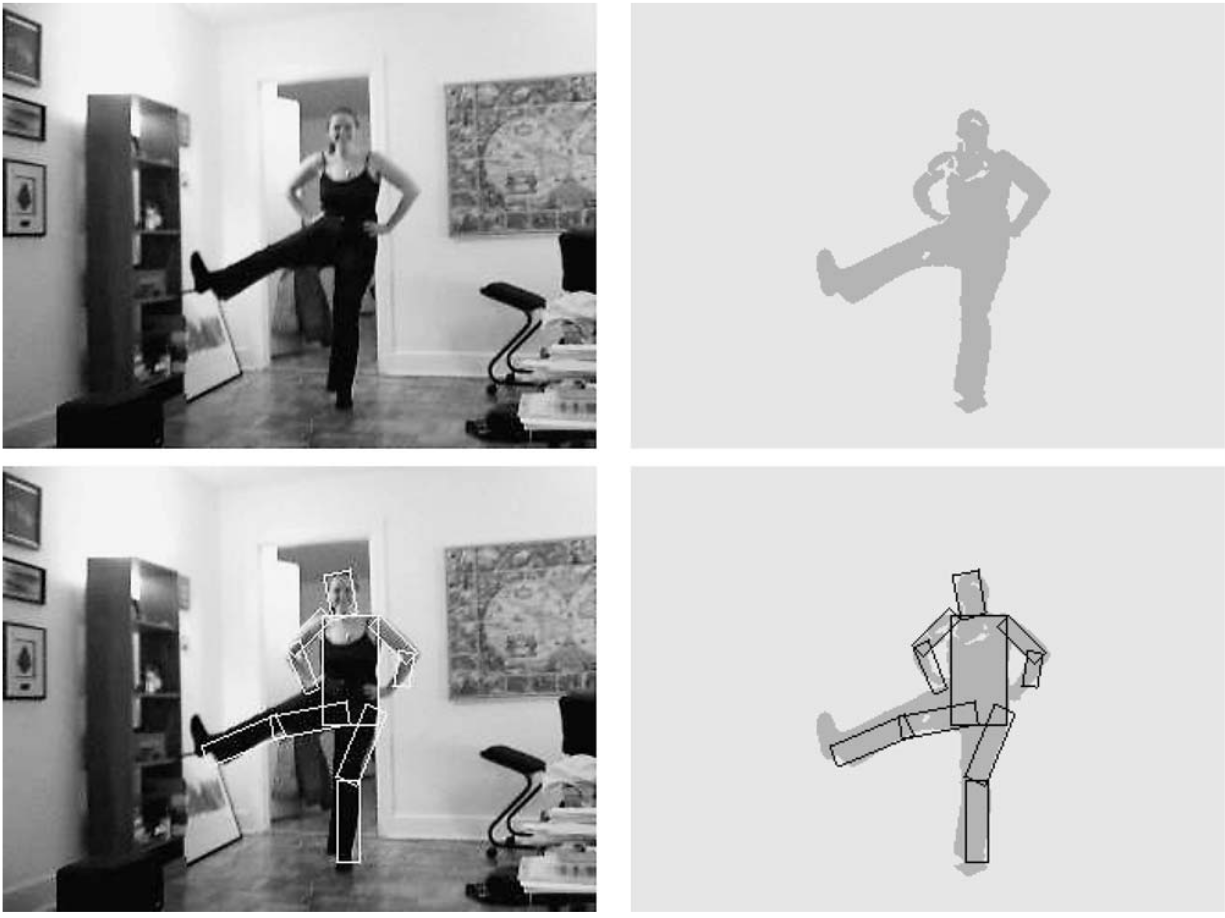
\includegraphics[width=0.8\textwidth]{felzenszwalb-overview.png}
    \caption{Overview of pose matching algorithm. \textbf{Upper left}: Original image. \textbf{Upper right}: binary image where foreground pixels (containing the human figure) are separated from the background. \textbf{Lower right}: One result from matching the limb rectangles to maximize the amount of foreground pixels covered. \textbf{Lower left}: Final result with estimated pose layered on top of original image. Image taken from \cite{felzenszwalb_pictorial_2005}.}
    \label{fig:felzenszwalb-overview}
\end{figure}

The authors model the human pose as a collection of $10$ different parts. 
Two parts per arm and leg as well as one torso and one head part \fref{fig:felzenszwalb-overview}.
Each part configuration $l_i = (x_i, y_i, s_i , \varphi_i)$ contains the $x$ and $y$ coordinate of the center of the rectangle representing the part.
In addition, $s_i \in [0,1]$ defines the length of the rectangle and $\varphi_i$ its rotation.
The width is fixed.

To model $p(I \mid l_i, \theta_i)$ they use the formula in \eref{eq:felz-unary} which utilizes $\theta_i = (q_1, q_2)$.
$q_1$ is the probability of pixel inside $l_i$ being a foreground pixel whereas $q_2$ is the probability of pixels closely around $l_i$ being foreground pixels.
The area around $l_1$ is referred to as $area_2$ whereas the area of $l_i$ is referred to as $area_1$.
$count_i$ referres to the number of foreground pixels in $area_i$ and $t$ is the total number of pixels in the image.

\begin{equation}
    \label{eq:felz-unary}
    \begin{split}
        p(I \mid l_i, (q_1, q_2)) = &q_1^{count_1} * (1 - q_1)^{(area_1 - count_1)} \\ 
        &* q_2^{count_2} * (1 - q_2)^{(area_2 - count_2)} \\ 
        &* 0.5^{(t - area_1 - area_2)}
    \end{split}
\end{equation}

Also, they smooth the distribution to prevent peaks by using the principle of annealing with a constant factor $T$ \eref{eq:smoothed}.
This is important because a distribution with strong peaks is more likely to return similar results when sampled from.
As discussed earlier, sampling is needed because of the approximation of the unary term the authors used and its problem with overlapping limbs.
A distribution with too strong peaks would not allow for sufficiently different pose samples.

$\theta_i$ is then estimated using mean values from annotated training data points while $T$ is set to $10$.

\begin{equation}
    \label{eq:smoothed}
    p(I \mid l_i, \theta_i) \propto p(I \mid l_i, \theta_i)^{\frac{1}{T}}
\end{equation}

\begin{figure}[htb!]
    \centering
    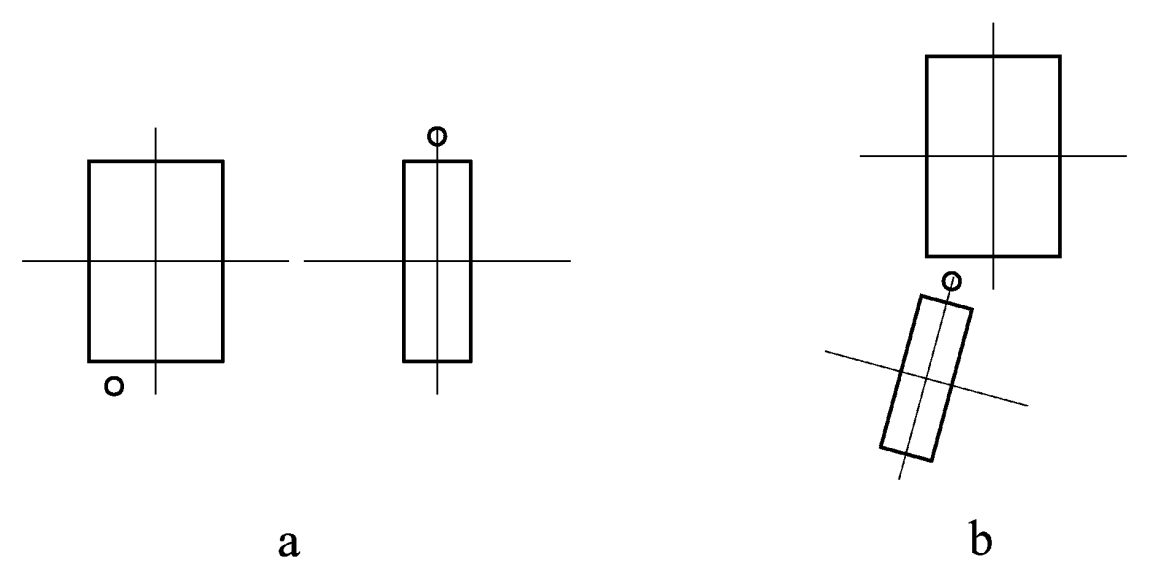
\includegraphics[width=0.8\textwidth]{limb-connection.png}
    \caption{Visualization of connecting limbs. \textbf{a}: Two limbs in their own coordinate system. The circles indicate connection joints. \textbf{b}: Possible, anatomically plausible connection. Image taken from \cite{felzenszwalb_pictorial_2005}.}
    \label{fig:limb-connection}
\end{figure}

Next, the authors model the prior $p(L \mid \theta)$.
Each spatial relation $p(l_i, l_j \mid \theta)$ between two parts is modelled in the following way:
First, each part is placed inside its own coordinate system with the origin being the center point of the part (see Figure \ref{fig:limb-connection}a).
The connection point (joint) between parts $i$ and $j$ is defined as $(x_{ij}, y_{ij})$ in the coordinate system of part $i$ and as $(x_{ji}, y_{ji})$ in the coordinate system of part $j$.
When transformed to the image coordinate system, these points should be as close together as possible (see Figure \ref{fig:limb-connection}b).
The authors express this using Gaussian distributions:

\begin{equation}
    \begin{split}
        N((\hat{x}_i - \hat{x}_j), 0, \sigma^2_x) \\
        N((\hat{y}_i - \hat{y}_j), 0, \sigma^2_y),       
    \end{split}
\end{equation}

where $\hat{x}_i$ and $\hat{y}_i$ are transformations of the joint position into the image coordinate system:

\begin{equation}
    \begin{bmatrix}
        \hat{x}_i \\ 
        \hat{y}_i
    \end{bmatrix}
    =
    \begin{bmatrix}
        x_i \\ 
        y_i
    \end{bmatrix}
    + s_i R_{\varphi_i}
    \begin{bmatrix}
        x_{ij} \\ 
        y_{ij}
    \end{bmatrix}.
\end{equation}

$\hat{x}_j$ and $\hat{y}_j$ are computed analogously.
$R_{\varphi_i}$ is a matrix which rotates around the origin for $\varphi_i$ radiants.
Additionaly, the authors define that the difference between $s_i$ and $s_j$ should be close to zero as well.
Again, this is modelled using a Gaussian distribution:

\begin{equation}
    N((s_i - s_j), 0, \sigma^2_s).
\end{equation}

Lastly, the authors specify that the difference between the two relative angles $\varphi_i$ and $\varphi_j$ be close to a parameter $\varphi_{ij}$.
They use a von Mises distribution, given by

\begin{equation}
    M(\theta, \mu, k) \propto \exp (k \cdot \cos (\theta - \mu)).
\end{equation}

A von Mises distribution can be thought of as a normal distribution around a circle, which is why the authors use it for periodic input like gradients.
Using $\mu = \varphi_{ij}$ they specify the constrained described earlier.
The parameter $k$ determines how strong the peak at $\varphi_{ij}$ should be or, in other words, how constrained the joints should be.

In summary, each spatial relation is expressed in the following way:

\begin{equation}
    \begin{split}
        p(l_i, l_j \mid \theta) 
        &= p(l_i, l_j \mid c_{ij}) \\
        &= N((\hat{x}_i - \hat{x}_j), 0, \sigma_x^2) \\
        &* N((\hat{y}_i - \hat{y}_j), 0, \sigma_y^2) \\
        &* N((s_i - s_j), 0, \sigma_s^2) \\
        &* M((\varphi_i - \varphi_j), \varphi_{ij}, k).
    \end{split}    
\end{equation}

Except for the last part of the equation, all distributions are Gaussian with a mean of $0$.
The last distribution is a von Mises distribution, given by

\begin{equation}
    M(\theta, \mu, k) \propto \exp (k \cdot \cos (\theta - \mu)).
\end{equation}

A von Mises distribution can be thought of as a normal distribution around a circle, which is why the authors use it for periodic input like gradients.
Using this distribution, the difference between the two angles is measured with regards to the optimal orientation $\varphi_{ij}$.
The parameter $k$ determines how strong the peak at $\varphi_{ij}$ should be or, in other words, how constrained the joints should be. 

The prior parameters $c_{ij}$ are then given by $c_{ij} = (x_{ij}, x_{ji}, y_{ij}, y_{ji}, \sigma_x, \sigma_y, \sigma_s, \varphi_{ij}, k)$ and are estimated using maximum likelihood estimation.

% ----- Short evaluation
The authors merely provide example images instead of a quantitative analysis.
This is most likely because of the lack of benchmark data sets available at the time.
They labeled $10$ images by hand and used these to estimate the parameters.
Then, for each of their unlabeld test images, they sampled $200$ poses and calculated the Chamfer distance, which measures the binary correlation.
The best pose with regards to the Chamfer distance is then returned.
Some example images can be seen in \fref{fig:pictoral-examples}

\begin{figure}[htb!]
    \centering
    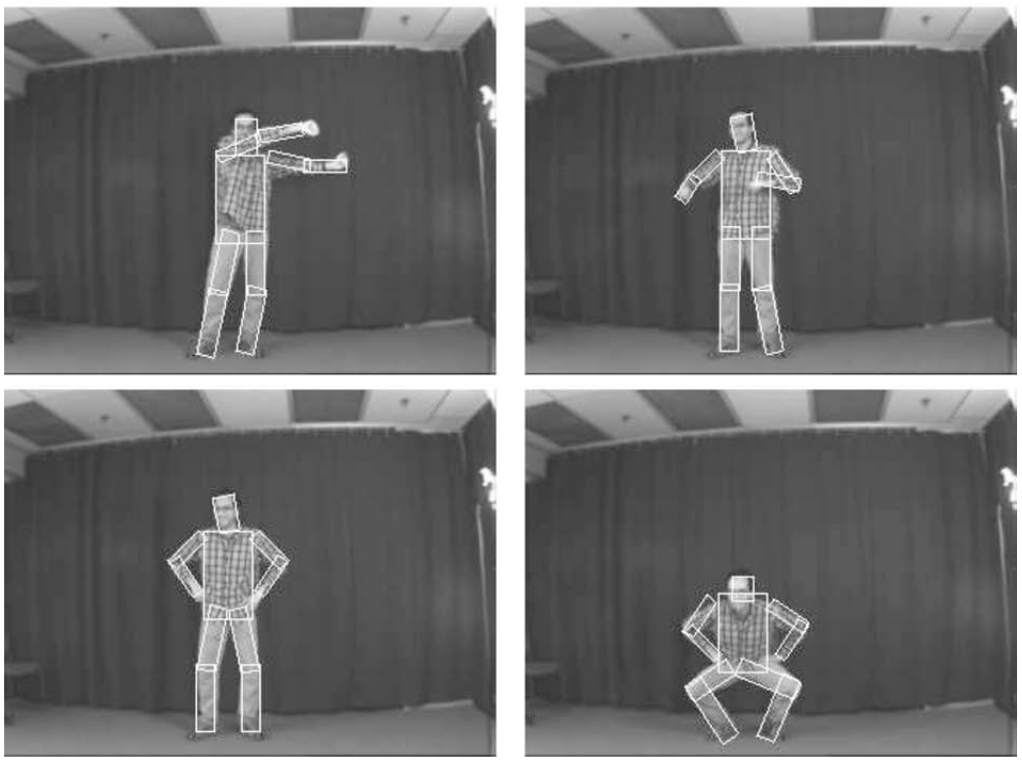
\includegraphics[width=0.8\textwidth]{pictoral-examples.png}
    \caption{Example of poses estimated by the statistical framework. Image taken from \cite{felzenszwalb_pictorial_2005}.}
    \label{fig:pictoral-examples}
\end{figure}

\subsubsection{Pictoral structures revisisted}

\subsubsection{Articulated pose estimation with flexible mixture-of-parts}

\begin{itemize}
    \item Articulated pose estimation with flexible mixture-of-parts \cite{yang_articulated_2011}
    \item An approach to pose-based action recognition \cite{wang_approach_2013}
\end{itemize}

\subsection{Deep Learning Methods}
% Deep Pose

- regresses joint coordinates (normalized)
- (illustrate architecture and explain where they got it from \cite{krizhevsky_imagenet_2012})
- local response normalization  
    - relu is unrestricted. some normalization is preferred because it makes the net generalize better \cite{krizhevsky_imagenet_2012}. applied after relu.
    - normalization between channels
    - no explanation (in \cite{krizhevsky_imagenet_2012}) given of why it works
- uses cascades. something we will see again in deep methods.
    - each stage is supposed to refine the prediction of the previous stage.
    - cut bounding box around previous prediction. Each stage gets a different "view". also: normalize to bounding box diameter

\subsubsection{DeepPose}
% Introduction
One of the first approaches for pose estimation using deep convolutional neural networks was proposed by \cite{toshev_deeppose:_2014}.
They achieved state-of-the-art results on two benchmark datasets using a neural network architecture based on the ImageNet network \cite{krizhevsky_imagenet_2012}.
In contrast to the pictoral structure framework discussed earlier, the approach was to regress the image coordinates directly without specific constrains on how the joints are allowed to be connected.

% Architecture
The authors define their network in terms of multiple connected \textit{stages}.
Each \textit{stage} is comprised of the neural network architecture proposed by \cite{krizhevsky_imagenet_2012}.
The used architecture is provied in Table \ref{tab:deeppose-architecture}.
The only change the authors made was to use the output of the last fully connected layer to regress the joint coordinates as opposed to the softmax activation present in \cite{krizhevsky_imagenet_2012}.
This means that, assuming $k$ joints, the output of a stage is of size $2 * k$.
Stage $s_0$ is trained using the full images of size $220 x 220$ as its input.
Once the first stage is trained until convergence, the authors use the output coordinates to crop sub images around the initially predicted joint coordinates.
By feeding these subimages into another stage $s_1$ they argue that the predictions get more precise because local context becomes more important.
This cascading approach is then repeated with the next stages.
In the end, they use $3$ stages $S = (s_0, s_1, s_2)$ after evaluating different numbers of stages on a held-out training set.

\begin{table}[]
    \begin{tabular}{|l|l|l|l|l|}
    \hline
    \textbf{nr.} & \textbf{layer type} & \textbf{filter size} & \textbf{nr. of filters / neurons} & \textbf{stride} \\ \hline
    1 & convolutional & 11 x 11 x 3 & 96 & 4 \\
    2 & local response normalization &  &  &  \\
    3 & pooling & 3 x 3 &  & 2 \\ \hline
    4 & convolutional & 5 x 5 x 48 & 256 & 1 \\
    5 & local response normalization &  &  &  \\ 
    6 & pooling & 3 x 3 &  & 2 \\ \hline
    7 & convolutional & 3 x 3 x 256 & 384 & 1 \\
    8 & convolutional & 3 x 3 x 192 & 384 & 1 \\
    9 & convolutional & 3 x 3 x 192 & 256 & 1 \\ \hline
    10 & fully connected &  & 4096 &  \\
    11 & fully connected &  & 4096 &  \\ \hline
    12 & fully connected &  & 2k &  \\ \hline
    \end{tabular}
    \caption{One \textit{stage} of the DeepPose network. Architecture based on \cite{krizhevsky_imagenet_2012}.}
    \label{tab:deeppose-architecture}
\end{table}

% Evaluation
\begin{figure}[htb!]
    \centering
    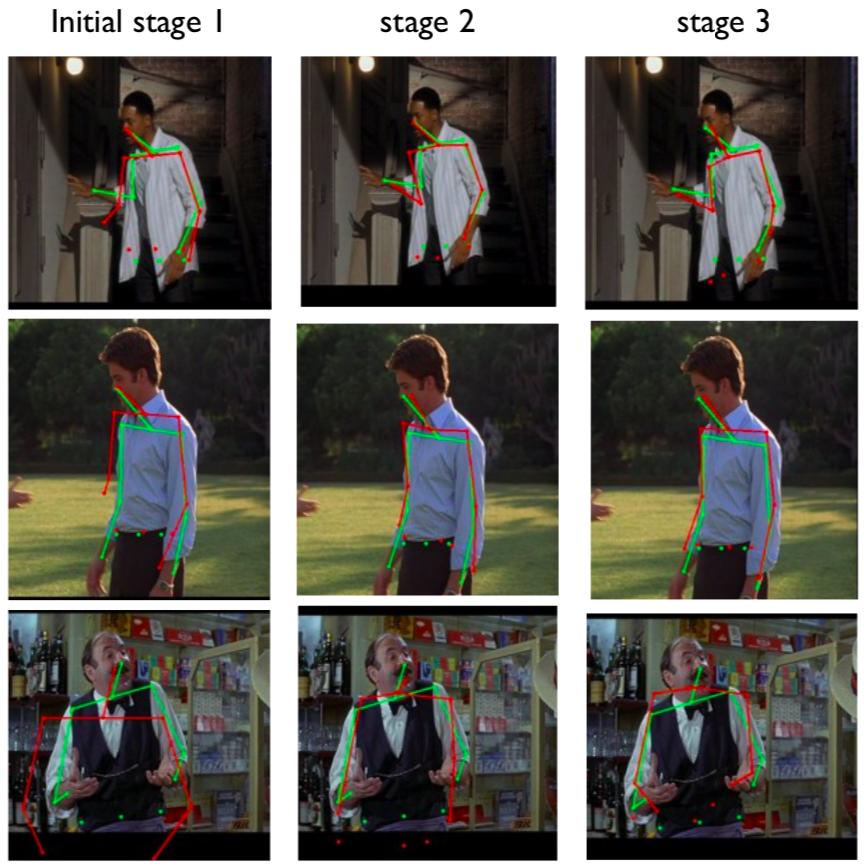
\includegraphics[width=0.5\textwidth]{deeppose-qualitative.png}
    \caption{Qualitative evaluation of the cascading architecture. Ground truth joints are shown in green while predicted poses are shown in red. Notice how the pose gets more accurate with consecutive stages. Also, notice that the biggest improvement can be seen after stage $1$. The authors argue that this is due to the fact that, with an increase in stages, the subimage gets smaller and smaller and thus harder to estimate the pose. Image taken from \cite{toshev_deeppose:_2014}.}
    \label{fig:deeppose-qualitative}
\end{figure}

% TODO: Move dataset / metric explanation if happening before
After training their network, the authors evaluate the final model on two datasets, FLIC \cite{sapp_modec:_2013} and LSP \cite{johnson_clustered_2010}.
Frames Labled In Cinema (FLIC) is a dataset which contains $5000$ images of Hollywoord movie scenes where $10$ upper body joint positions are labeled for the subject of the scene.
Leeds Sports Pose (LSP) is a dataset of $2000$ annotated images of subjects in a sport context.
LSP contains $14$ different joint positions of the entire body.

The authors use two different metrics to evaluate their model.
Percentage of Correct Parts (PCP) \cite{eichner_articulated_2010} meassures the detection rate of limbs instead of joint coordinates.
To still use this widely accepted metric, the authors take the ground truth coordinates of the joints on the end of each limb to calculate the limb length.
Then, when evaluating a predicted pose, a joint is defined as being detected correctly if the distance between the joint coordinate in the prediction and the ground truth is less than or equal to half of the limbs length.

PCP has the disadvantage that short limbs get penalized more than big limbs.
To overcome these shortcommings, the authors define a new evaluation metric called Percent of Detected Joints (PDJ).
With this metric, a joint is considered detected correctly if the distance between the predicted joint position and the ground truth $d_p$ is smaller than a fraction of the torsos diameter $d_t$.
This fraction is set to be $0.5$, meaning a joint is considered detected if $0 <= d_p <= 0.5 \cdot d_t$.

The authors provide three examples which illustrate the importance of the cascading architecture.
These examples can be seen in \fref{fig:deeppose-qualitative}.
They argue that stage $s_1$ has the biggest effect on the accuracy of the joints since further stages use smaller and smaller subimages for regression and thus use a smaller context.

\begin{itemize}
    \item DeepPose \cite{toshev_deeppose:_2014}
    \item Stacked Hourglass \cite{newell_stacked_2016}
    \item Convolutional Pose Machine \cite{wei_convolutional_2016}
    \item Thin-Slicing Network \cite{song_thin-slicing_2017}
\end{itemize}

\section{Video-based Human Action Recognition}
\subsection{Shallow Methods}
\begin{itemize}
    \item Learning Realisitic Human Actions from Movies \cite{laptev_learning_2008}
\end{itemize}

\subsection{Deep Methods}
\begin{itemize}
    \item MiCT \cite{zhou_mict:_2018}
\end{itemize}